\subsection{Baseline model}\label{baseline_model}

Before defining the neural networks in this work, a study of other similar work and results has been carried out and can be seen in section \ref{similar_projects}. This allows us to use the results of other projects as a reference point, knowing whether the development of this practice is improving the results obtained by other projects or not. In addition to having the points of reference of other projects, a base model has been defined.
\newline

A base model is a trivial model that is usually developed when you want to solve a prediction or classification problem in order to know if the other models to be developed will improve the result. In this project, the base model developed does not have logic and simply returns the value that existed one week before as a prediction.  
\newline

Below you can see graphically the model's predictions with respect to the real values:
\begin{figure}[H]
    \centering
    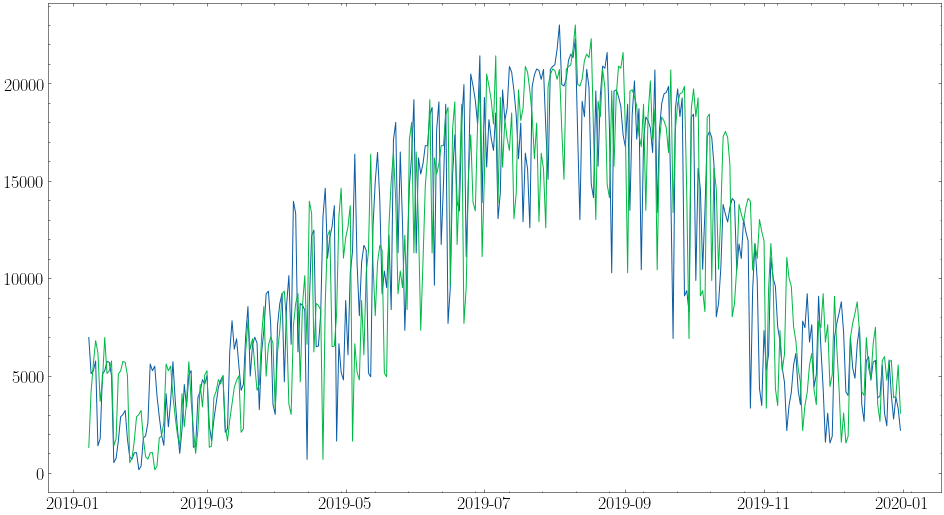
\includegraphics[width=16cm]{images/solution/predictions/baseline-predictions.png}
    \caption{Predictions of the basic model}
    \label{fig:baseline-predictions}
\end{figure}

It can be seen that the predictions are the same real values but displaced by a week. Once this model has been developed, the metrics shown in section \ref{results} have been calculated together with the rest of the results of the other models.
